



\documentclass[
	% -- opções da classe memoir --
	12pt,				% tamanho da fonte
	openright,			% capítulos começam em pág ímpar (insere página vazia caso preciso)
	oneside,			% para impressão em recto e verso. Oposto a oneside
	a4paper,			% tamanho do papel. 
	% -- opções da classe abntex2 --
	%chapter=TITLE,		% títulos de capítulos convertidos em letras maiúsculas
	%section=TITLE,		% títulos de seções convertidos em letras maiúsculas
	%subsection=TITLE,	% títulos de subseções convertidos em letras maiúsculas
	%subsubsection=TITLE,% títulos de subsubseções convertidos em letras maiúsculas
	% -- opções do pacote babel --
	english,			% idioma adicional para hifenização
	french,				% idioma adicional para hifenização
	spanish,			% idioma adicional para hifenização
	brazil				% o último idioma é o principal do documento
	]{abntex2}




% Pacotes básicos 
\usepackage{lmodern}			% Usa a fonte Latin Modern			
\usepackage[T1]{fontenc}		% Selecao de codigos de fonte.
\usepackage[utf8]{inputenc}		% Codificacao do documento (conversão automática dos acentos)
\usepackage{indentfirst}		% Indenta o primeiro parágrafo de cada seção.
\usepackage{color}				% Controle das cores
\usepackage{graphicx}			% Inclusão de gráficos
\usepackage{microtype} 			% para melhorias de justificação
\usepackage{amsmath}			% lib para equacoes
\usepackage{svg}
\usepackage{pythonhighlight}
%\usepackage{float}


% Pacotes adicionais, usados apenas no âmbito do Modelo Canônico do abnteX2

\usepackage{lipsum}				% para geração de dummy text



% Pacotes de citações
\usepackage[num, backend=biblatex]{abntex2cite}	% Citações padrão ABNT
\usepackage[brazilian,hyperpageref]{backref}	 % Paginas com as citações na bibl


 
% CONFIGURAÇÕES DE PACOTES

% Configurações do pacote backref
% Usado sem a opção hyperpageref de backref
\renewcommand{\backrefpagesname}{Citado na(s) página(s):~}
% Texto padrão antes do número das páginas
\renewcommand{\backref}{}
% Define os textos da citação
\renewcommand*{\backrefalt}[4]{
	\ifcase #1 %
		Nenhuma citação no texto.%
	\or
		Citado na página #2.%
	\else
		Citado #1 vezes nas páginas #2.%
	\fi}%
% ---



% ---
% Informações de dados para CAPA e FOLHA DE ROSTO
% ---
\titulo{Robô omnidirecional de 3 rodas}
\autor{Daniel Ermelino Carvalho \\ Lucas Pereira Lima}
\local{Brasil}
\data{2022}
\orientador{Marcelo Bender Perotoni}
\instituicao{%
  Universidade Federal do ABC
  \par
  CECS
  \par
   Engenharia de Instrumentação, Automação e Robótica}
\tipotrabalho{Tese (Doutorado)}
% O preambulo deve conter o tipo do trabalho, o objetivo, 
% o nome da instituição e a área de concentração 
\preambulo{ }



% Configurações de aparência do PDF final

% alterando o aspecto da cor azul
\definecolor{blue}{RGB}{5,5,180}

% informações do PDF
\makeatletter
\hypersetup{
     	%pagebackref=true,
		pdftitle={\@title}, 
		pdfauthor={\@author},
    	pdfsubject={\imprimirpreambulo},
	    pdfcreator={LaTeX with abnTeX2},
		pdfkeywords={abnt}{latex}{abntex}{abntex2}{trabalho acadêmico}, 
		colorlinks=true,       		% false: boxed links; true: colored links
    	linkcolor=blue,          	% color of internal links
    	citecolor=blue,        		% color of links to bibliography
    	filecolor=magenta,      		% color of file links
		urlcolor=blue,
		bookmarksdepth=4
}
\makeatother


% Posiciona figuras e tabelas no topo da página quando adicionadas sozinhas
% em um página em branco. Ver https://github.com/abntex/abntex2/issues/170
\makeatletter
\setlength{\@fptop}{5pt} % Set distance from top of page to first float
\makeatother



% Possibilita criação de Quadros e Lista de quadros.
% Ver https://github.com/abntex/abntex2/issues/176

\newcommand{\quadroname}{Quadro}
\newcommand{\listofquadrosname}{Lista de quadros}

\newfloat[chapter]{quadro}{loq}{\quadroname}
\newlistof{listofquadros}{loq}{\listofquadrosname}
\newlistentry{quadro}{loq}{0}

% configurações para atender às regras da ABNT
\setfloatadjustment{quadro}{\centering}
\counterwithout{quadro}{chapter}
\renewcommand{\cftquadroname}{\quadroname\space} 
\renewcommand*{\cftquadroaftersnum}{\hfill--\hfill}

\setfloatlocations{quadro}{hbtp} % Ver https://github.com/abntex/abntex2/issues/176


% Espaçamentos entre linhas e parágrafos 


% O tamanho do parágrafo é dado por:
\setlength{\parindent}{1.3cm}

% Controle do espaçamento entre um parágrafo e outro:
\setlength{\parskip}{0.2cm}  % tente também \onelineskip


% compila o indice
\makeindex




% Início do documento
\begin{document}

% Seleciona o idioma do documento (conforme pacotes do babel)
%\selectlanguage{english}
\selectlanguage{brazil}

% Retira espaço extra obsoleto entre as frases.
\frenchspacing 


% ELEMENTOS TEXTUAIS
\textual

	% Capitulo com exemplos de comandos inseridos de arquivo externo 
	\include{abntex2-modelo-include-comandos}

	\chapter{Projeto 1}
		Daniel Ermelino Carvalho - RA 11092613
		
		Elton Mauricio Da Silva - RA 11201810955

		link de arquivos: \url{https://github.com/dcarve/data_visulization_ufabc}
	
	\chapter{Questao 1}

\subsection*{Código}

\begin{python}
import pandas as pd
import numpy as np
import matplotlib

# pre convertido para utf-8
df = pd.read_csv('VIS_Pr_01_Vendas.csv')

df = df.groupby('Region').agg(
    {
        'Sales': ['sum'],
        'Profit': ['sum'],
        'Discount': ['mean']     
    }
).reset_index()


df.columns = ["_".join(t).strip('_') for t in df.columns]

#exportando csv configuracoes do MS excel
df.to_csv(
    'result_q1.csv',
    sep=';',
    index=False,
    encoding='utf-8-sig'
)
\end{python}

\subsection*{Output file}


\begin{quadro}[htb]
	\caption{File - result\_q1.csv }
    \begin{tabular}{|l|l|l|l|}
		\hline
        Region & Sales\_sum & Profit\_sum & Discount\_mean \\ \hline
        Central&501239.8908&39706.3625&0.24035299182092124 \\ \hline
        East&678781.24&91522.78&0.14536516853932585 \\ \hline
        South&391721.905&46749.4303&0.1472530864197531 \\ \hline
        West&725457.8245&108418.4489&0.10933499843896347 \\ \hline
	\end{tabular}
	\end{quadro}

\subsection*{Comentários}
 O arquivo veio com o encoder ANSI, que é proprietário da Microsoft, o que atrapalha a leitura no linux, logo o arquivo tem que ser converdito para um outro encoder,
 no caso, o arquivo foi convertido para utf-8.
 No windows, o arquivo pode ser lido usando pd.read\_csv('VIS\_Pr\_01\_Vendas.csv', encoding='ansi'), mas não funcionaria no linux.
 Já a exportação do arquivo, a configuração nativa de csv usado no excel, é com separador ";" e o encoder tem que ser utf-8-sig.

	\chapter{Questao 2}

\subsection*{Código}

\begin{python}
import pandas as pd
import numpy as np
import matplotlib.pyplot as plt

# pre convertido para utf-8
df = pd.read_csv('VIS_Pr_01_Vendas.csv')

df['order_year'] = pd.to_datetime(df['Order Date']).dt.strftime('%Y')

df = df.groupby(['Sub-Category','order_year']).agg(
    {'Profit': ['sum']}
).reset_index()

df.columns = [
    "_".join(t).strip('_').replace('-','_').lower()
    for t in df.columns
]

df = df.pivot(
    index='sub_category',
    columns='order_year',
    values=['profit_sum']
).reset_index()

df.columns = [
    (t[1] if ('profit_sum' in t) else t[0])
    for t in df.columns
]

sub_category = df['sub_category'].to_list()
values = df.drop('sub_category', axis=1).to_dict('list')


x = np.arange(len(sub_category))
width = 0.15
multiplier = 0

fig, ax = plt.subplots(
    constrained_layout=True,
    figsize=(15, 7)
)

for attribute, measurement in values.items():
    
    rgb = (
        (12*(5**(-multiplier))*(10**multiplier))/255,
        (34+(45*multiplier))/255,
        (150+(30*multiplier))/255,
    )    
    
    offset = width * multiplier
    rects = ax.bar(
        x + offset,
        measurement,
        width,
        label=attribute,
        color=rgb)
        
    multiplier += 1

ax.set_ylabel('profit')
ax.set_xticks(x + width, sub_category)
ax.legend(loc='upper left')
ax.grid(axis = 'y')

plt.show()'
\end{python}


\subsection*{plot}
\begin{figure}[h]
	\centering
	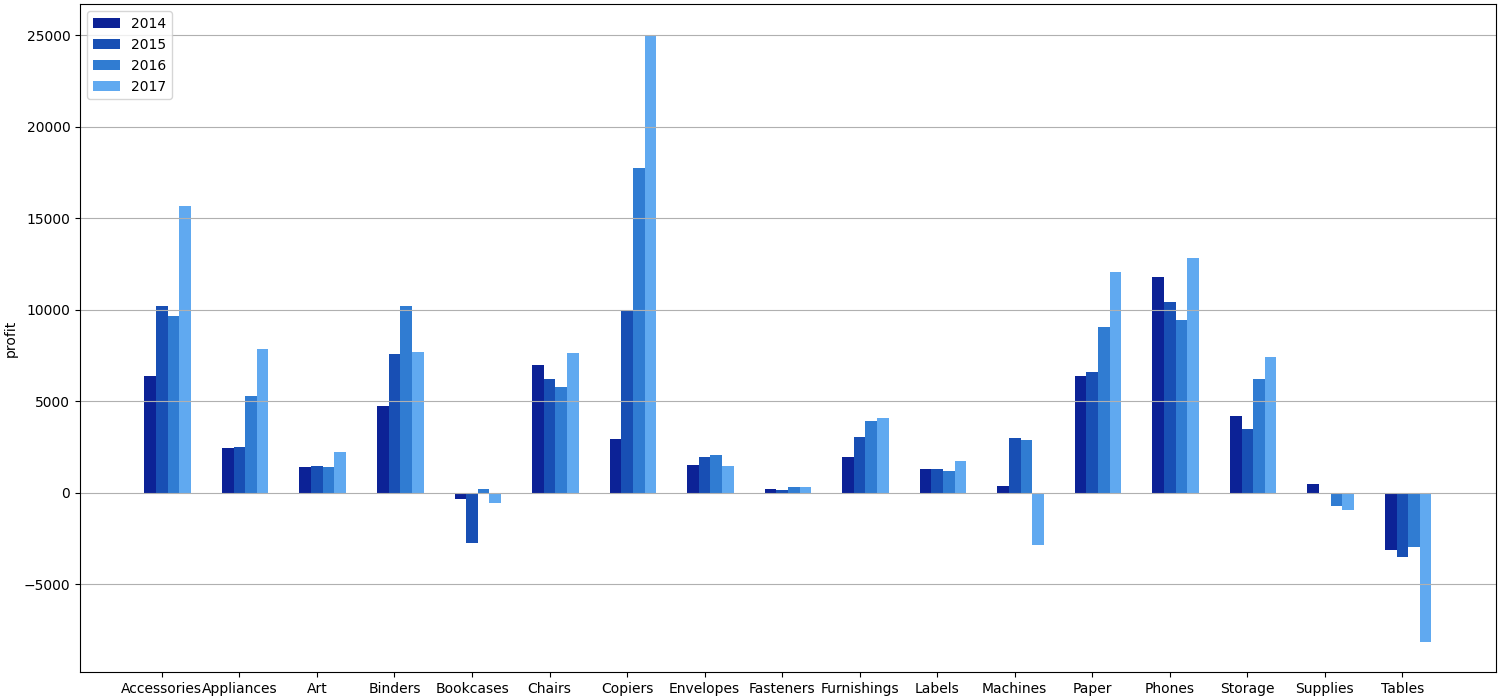
\includegraphics[width=\textwidth,keepaspectratio]{figures/graph_bar}
	\caption{diagrama do modelo - dedução da matriz}
	\label{lof}
\end{figure}

\subsection*{Comentários}
Os gráficos do matplotlib embora podem ser facilmente personalizados,
exigem um código mais extenso para o caso de houver mais dados e quiser manter a personalização de esquemas de cores do gráfico.

	\chapter{Questao 3}

\subsection*{Código}

\begin{python}
import pandas as pd

# pré convertido para utf-8
df = pd.read_csv('VIS_Pr_01_Vendas.csv')

df = df.copy()

df['perform']  = df['Profit']/(df['Sales']-df['Discount'])

df = df.groupby(['Customer Name', 'Segment']).agg(
    {'perform': ['mean']}
).reset_index()

df.columns = [t[0] for t in df.columns]


def f(x):
    
    if x<0.1:
        return "E"
    elif (x>-0.1) and (x<0.15):
        return "D"
    elif (x>-0.15) and (x<0.2):
        return "C"
    elif (x>-0.2) and (x<0.25):
        return "B"
    elif (x>-0.25):
        return "A"


df['perform'] = df.apply(
    lambda row: f(row['perform']),
    axis=1
)


#exportando csv configurações do MS excel
df.to_csv(
    'result_q3.csv',
    sep=';',
    index=False,
    encoding='utf-8-sig'
)
    
\end{python}


\subsection*{Output file}


\begin{quadro}[htb]
	\caption{File - result\_q23.csv}
    \begin{tabular}{|l|l|l|}
		\hline
        Customer Name & Segment & perform \\ \hline
        Aaron Bergman & Consumer & D \\ \hline
        Aaron Hawkins & Corporate & A \\ \hline
        Aaron Smayling & Corporate & E \\ \hline
        Adam Bellavance & Home Office & A \\ \hline
        Adam Hart & Corporate & C \\ \hline
        Adam Shillingsburg & Consumer & E \\ \hline
        Adrian Barton & Consumer & E \\ \hline
        ... & ... & ... \\ \hline
        Zuschuss Carroll & Consumer & E \\ \hline
        Zuschuss Donatelli & Consumer & A \\ \hline
	\end{tabular}
	\end{quadro}

\subsection*{Comentários}
Esse é caso em que falta é necessário supor algumas informação.
após fazer a conta de performance, para os caso de houver mais de uma categoria vendida por consumidor, o resultado da performance é uma soma ou média?
Nesse caso foi suposto uma média, pois faria mais sentido com as condições estabelecidas depois, em que converte o valor da performance em letras de "A" a "E"


	% ----------------------------------------------------------
	% Finaliza a parte no bookmark do PDF
	% para que se inicie o bookmark na raiz
	% e adiciona espaço de parte no Sumário
	% ----------------------------------------------------------
	\phantompart

%---------------------------------------------------------------------
% INDICE REMISSIVO
%---------------------------------------------------------------------
\phantompart
\printindex


\end{document}

